\chapter{Architecture of a Network Device}
\label{chap:architectureOfNetworkDevice}

\begin{chapterintro}
% Napsat o tom, ze v teto casti rozebereme cilovou architekturu, kterou je FPGA a na to budeme mapovat nase sitove zarizeni
In this chapter, we introduce possible target architectures for mapping of P4 program. 
Namely, we introduce details about state-of-the-art software implementations capable 
to process 10\,Gbps, Network Processing Units (NPUs) capable to process traffic at speed of 40\,Gbps and beyond. The text also provides details about
Field Programmable Gate Array (FPGA) which is a common platform for implementation of high-speed network hardware. 
Finally, this chapter proposes our architecture of high-speed processing pipeline which is suitable for mapping from the abstract description.
\end{chapterintro}

\section{Target Architectures}
This section introduces the most common target platforms for implementation of network applications. We introduce software based targets in the 
beginning of the text. Then, we continue with introduction of hardware based targets which are suitable for processing of high-speed network
traffic.

%\subsection{Possible Target Architectures}
%\label{sec:possibleTargetArchitectures}

\subsection*{CPU}
The most common target is a software tool for ordinary Central Processing Units (CPUs). 
Such solutions are commonly used because they are flexible and easy to deploy with minimal 
cost. Moreover, computers can be connected to a large and powerful cluster which is capable to process high-speed network streams. 
The disadvantage of this approach is poor scalability for processing of network data in real time.

Pedro et al. \cite{SantiagodelRioWireSpeedCommodityHw}
introduce the solution for analysis of 10\,Gbps traffic on commodity hardware with slightly modified network drivers. 
The target architecture is able to fully classify incoming traffic at speed of 14.2 milion packet per second (Mpps). 
However, the paper doesn't present any possibility for generation of processing program from abstract description.

Marian et al. \cite{MarianNetSlicesUserDefinedProcess} introduce the NetSlice operating system abstraction which 
tightly couples the hardware and software packet processing resources. 
The NetSlice performs domain specific, spatial partitioning of system resources like CPU cores, memory and NIC. 
It also provides a special low latency channel between NIC and user-space application. 
Using this approach, the user-space application is capable to receive and process network traffic at speed of 10\,Gbps.

CLICK \cite{kohler2000click} is the domain specific language and set of modules for implementation
of network applications. The language defines a unified interface for easy connection of all modules
which are organized in directed dataflow graph. Modules are capable to construct and modify protocol fields
of processed packets. This solution can be easily extended to support new protocol sets. However, this tool is implemented
in software which doesn't make it suitable for using in high-performance networks. 

The P4 language consortium introduces the P4-HLIR library \cite{p4hlir} which is the front end of the P4 compiler, creating Python object model of the 
P4 program. It is useful for other projects because one can easily continue with implementation of compiler's back end from this object
representation. The P4C-BEHAVIORAL compiler \cite{p4cbeavioral} is the example of such implementation. It implements the back end for translation
from P4 language to C++.

\subsection*{NPU}
Another common architecture is the Network Processing Unit (NPU). It is an integrated circuit which has a specific feature set for network 
application domain. The example of this feature set can be fast and effective implementation of classification engines, pattern matching, 
data bitfield manipulation, and so on. 
The NPUs are typically software programmable and parallel devices with specialization on computer networks and telecommunications. 
The architecture of network processors can be described in many ways. An extended general framework for classifying network processors was suggested in 
\cite{giladi2008network} including these five dimensions: 
(1) Parallel processing approach, (2) Hardware assistance (coprocessors for variety of optimized tasks), 
(3) Network processor interconnection mechanisms (e.g., on-chip communications), (4) Peripherals, 
(5) Flynn typology of multiprocessing (SIMD, SISD, MIMD, MISD). 
The disadvantage of this approach is the limited set of instructions/actions which cannot be extended during 
run time (i.e., we have to emulate them in software). 
However, the NPUs are capable to process network traffic at speed of 40\,Gbps \cite{netronome-npu} and beyond in real time. 

\subsection*{FPGA}
The Field-Programmable Gate Array (FPGA) is a common target platform in these days. 
It is an integrated circuit which is used for rapid prototyping of hardware.
The structure (and thus behavior) of implemented hardware is defined using the Hardware Description Languages (HDL). 
This platform connects the performance of NPUs and flexibility of software solutions to one compact package 
(the FPGA is also called as a \textit{programmable hardware}). 
There are also available FPGA based NICs which are capable to process speeds from 10\,Gbps to 100\,Gbps 
(see \cite{combo-100g,netfpga} for further description).

\subsection{Detailed Description of FPGA}
\label{sec:fpgaTarget}
% Tady bude popis FPGA a mozna detaily o implementacni platforme (COMBO?)
FPGA is a semiconductor device whose structure can be reconfigured.
The configuration is specified using the HDL which is translated to bitstream (i.e., the configuration stream of FPGA). 
Simplified architecture of FPGA is shown in Fig.~\ref{fig:fpgaArch}. 

\begin{figure}[ht]
    \centering
    \includegraphics[scale=0.75]{chapters/pic/fpga}
    \caption{Simplified architecture of FPGA.}
    \label{fig:fpgaArch}
\end{figure}

The FPGA contains Configurable Logic Blocks (CLBs). These blocks are used as generators of logic functions and sequential logic.
The generator is realized by a memory which is configured with the truth table of implemented function --- Lookup Table (LUT) in terms of FPGA. 
The CLB also contains the gated D latch (i.e., one bit register) for implementation of sequential logic. 
Required behavior can be internally selected by multiplexer (e.g., we can select the register and enable the sequential behavior).
The brief scheme of CLB is shown in Fig.~\ref{fig:fpgaClb}. However, each vendor implements different features to CLB blocks.

The number of LUT inputs defines the row count of realized truth table ($2^n$ possible results for $n$ inputs). 
The most common number of LUT inputs is equal to four or six. Function with more variables is realized by connection of 
LUTs to a chain. FPGAs are often equipped with more specialized blocks like memories \cite{fpga-block-ram}, 
Digital Signal Processing (DSP) blocks \cite{fpga-dsp}, processors (like ARM) \cite{fpga-processor}, and so on. 
These embedded blocks have an influence on final frequency and used resources. 
For example, we can save CLB logic for implementation of memory or processor.
Each mentioned block communicate via configurable interconnection network. 

\begin{figure}[ht]
    \centering
    \includegraphics[scale=0.7]{chapters/pic/fpga-clb}
    \caption{Simplified architecture of CLB.}
    \label{fig:fpgaClb}
\end{figure}

The communication with external devices is performed via configurable input and output blocks. These blocks enable adaptation to external
signals and transfer them inside the FPGA. The high-speed communication can be performed via interfaces like 
RocketIO \cite{fpga-rocketio} (line rates up to 3.125\,Gbps), GTX/GTH \cite{fpga-gtx-gth} (line rates up 13\,Gbps), and so on. 
These high-speed communication interfaces can be used for attaching of Ethernet transceivers. 

Programmability of FPGAs make them suitable for the research in the area of computer networks because we can use an HDL language and describe
a complex behavior of hardware device. It is also used for fast prototyping of ASICs because developers can run and validate the chip's design
before production. This platform is also used by other researchers in this area for hardware acceleration of classification, packet parsing, and 
so on.
From provided description of FPGA, we feel that this target is very flexible and we can use it as a target platform
for implementation of a generic network device which is being generated from P4 source code.
The high-speed networking world offers many challenges regarding architectures and algorithms for implementation of network devices, 
capable to process traffic at speed of 100\,Gbps and beyond.
Moreover, the FPGA platform allows to accommodate different applications without any change of physical hardware. 
Therefore, we want to use the P4 language together with FPGA target for our research.

\section{Generic Architecture of a Network Device}
% Napsat cile, ze to bude sitove zarizeni generovane z abstraktniho popisu. Zakladni mozny pristup v paralelnim nebo pipelinovem zapojeni. 
% Pipelina bude lepsi, protoze nam bude umoznovat lepsi trade off mezi propustnosti a spotrebovanyma zdrojema.
% Dalsi deleni se uvidi

As we notice before, we chose the FPGA as the main implementation platform for generated devices from P4 description. 
This platform connects the flexibility of software and parallel nature of hardware together 
(i.e., the functionality of the hardware can be reprogrammed).
The initial idea of P4 device model was introduced in \cite{p4,p4languagespec,GibbPhd}. 
The text provides more details about this model in Sec.~\ref{sec:p4Model}.
Unfortunately, the P4 device model isn't suitable for some use cases because the match and action part is strictly defined. 
We propose the Parser-Deparser model which freely defines a functionality between parser and deparser blocks.
The text provides more details about this approach in Sec.~\ref{sec:parserDeparserModel}.
Finally, Sec.~\ref{sec:architectureOfProcessingPipeline} proposes the architecture of generic processing pipeline
which is suitable for accommodation of P4 hardware.  

\subsection{P4 Device Model}
\label{sec:p4Model}
% Popis parser-deparser pristupu (vykopirovat z MICPRO)
The P4 device model contains parser, deparser, Match+Action tables and queuing mechanism 
(see Fig.~\ref{fig:originalP4DeviceModel}).
The first module, parser, is used to break the incoming network data into individual header fields. These data fields are passed to 
the ingress Match+Action tables where packet modification and egress selection is performed. After that, the ingress Match+Action pipeline passes 
data to queuing mechanism which implements traffic distribution, based on configuration from ingress Match+Action tables. 
Egress Match+Action pipeline is used for final modification of protocol fields before deparsing, which is performed in the last module.
This module is used for construction of network packet back from the form of protocol headers. 
The proposed model is general enough for wide range of applications. 
However, it isn't able to implement another advanced architectures for processing of network traffic 
(like pattern matching or extended stateful processing).  

\begin{figure}[ht]
    \centering
    \includegraphics[width=11cm]{chapters/pic/P4DeviceModel.pdf}
    \caption{Model of P4 device (taken from \protect\cite{p4languagespec}).}
    \label{fig:originalP4DeviceModel}
\end{figure}

\subsection{Parser-Deparser Model}
\label{sec:parserDeparserModel}
Due to the disadvantage described above, we propose more general model which is based on free specification of processing part 
(simplified architecture is shown in Fig.~\ref{fig:parserDeparserArchitecture}). 
%Notice that processing part of original model consists of Ingress Match+Action, Queuing mechanism and Egress Match+Action pipeline.
Our model of network device is based on standard P4 model and it consists of three modules. 
The first module, parser, is used to break the incoming network data into individual header fields
(i.e., it has the same functionality like parser in P4 model).
The output of this module is a set of structured extracted fields and valid bits.
The valid bit is used for presence indication of extracted protocol fields in actually processed packet.
The structure of protocol fields is based on the P4's Header Format definition. 
All extracted protocol fields and valid bits are passed to the second module, process, 
which implements the general processing engine (e.g., VLAN tagging, Network Address Translation, Traffic analysis). 
This block implements the functionality of accelerated engine. It also sets a validity information for each inserted/not inserted protocol 
and filters out all unused header data (i.e., this data will not be used during packet assembling). 
Finally, the last module, deparser, is used for construction of network packet back from protocol headers and valid bits.
This approach is general enough for variety of network applications. The Parser-Deparser model is capable to accommodate the P4 device model 
because the Process part allows mapping of Ingress Match+Action, Queues and/or Buffers and Egress Match+Action to predefined general architecture. 
This work introduces possible mapping in Sec.~\ref{sec:architectureOfProcessingPipeline}.

\begin{figure}[t]
    \centering
    \includegraphics[width=\textwidth]{chapters/pic/ParserDeparserApproach}
    \caption{Parser-Deparser model.}
    \label{fig:parserDeparserArchitecture}
\end{figure} 

The VLAN tagging is a classic and common use case in many network applications. 
Tagging process consists of two main steps --- insertion of VLAN header to packet and setting of appropriate header field value of 
current Ehernet protocol.
In the case of Parser-Deparser model, the supported protocol stack is directly represented in the hardware device where each protocol
occupies one position on header and valid bus. 
Therefore, the VLAN tagging operation consists of setting of the VLAN header on header bus, setting of appropriate valid bit 
(i.e., header will be inserted) and setting of appropriate Ethernet header field value. Finally, the packet is assembled in the deparser block. 
 
The network traffic analysis is another common use case.
The analysis is based on investigation of data from extracted headers which are used 
as an input to analysis function. This function can be a general process like pattern matching, detection of malicious traffic, and so on. 
The Parser-Deparser model allows easy access to all extracted data in parallel because data are preprocessed in parser stage and put onto header
data lines. The traffic analysis algorithm is implemented in process module. This use case isn't easy to implement in standard P4 device model
because the structure and set of supported actions is predefined in P4 standard.

In this section, we proposed our Parser-Deparser model. The model can be partially generated from P4 description.
More precisely, we can generate the parser and deparser modules from the Header Format and Packet Parser definition, because both 
modules have homogeneous and general structure. Our Process block can be generated from P4, but is generic beyond what P4 describe.
In this work, we show the ability of our model. 
We use a P4 language as an input of transformation process which effectively maps the P4 source code to hardware representation.
The Parser-Deparser model is published in \cite{2016MicproP4}.

\subsection{Mapping P4 to Parser-Deparser Model}
\label{sec:architectureOfProcessingPipeline}

The following text brings details of the architecture of processing pipeline in Fig.~\ref{fig:p4PipelineArchitecture} 
(published in \cite{2016h2rc-p4}). 
The idea uses our Parser-Deparser model which was introduced in Sec.~\ref{sec:parserDeparserModel}. 
The \emph{parser} is used to break the incoming data to individual protocol header fields and payloads.
Our architecture also allows synchronization of outside metadata with parsed headers. 
The outside metadata are generated by input network buffer during receive of packet from network. 
This structure typically contains input port number and receive timestamp. The parsed headers and outside metadata are passed to the
\emph{metadata generator}. This block cooperates with parser on initialization of default metadata values.
The generated information is later used for advanced processing of parsed data in our pipeline 
(i.e., we can use metadata for controlling of functionality of processing elements).
Another output from \emph{parser} and \emph{metadata generator} is also the address of first active Match+Action processing 
element in \emph{Match+Action group}.

\begin{figure}[b]
    \centering
    \includegraphics[scale=0.9]{chapters/pic/IPv6MorePayloads}
    \caption{The example of packet with more payloads.}
    \label{fig:IPv6MorePayloads}
\end{figure}

All outputs (parsed headers, generated metadata, address of first \emph{Match+Action group} and parsed payloads) from \emph{parser} 
and \emph{metadata generator} are passed to 
\emph{check} module. This module performs validation of the checksum field of processed packet and setting of initial values of 
control path.
Some protocols need to be checked for validity of header or payload data because there may be errors during transfer through the network
(i.e., we need to detect this situation in processed protocol and pass this information to the pipeline). 
Our architecture supports processing of protocol with such specification. 
The example of protocol with checksum field is the Transmission Control Protocol (TCP) which is defined in \cite{rfc793-TCP}.
Initial values of control path signals are generated from result of the checksum validation, start table address, incoming protocol headers
and metadata values. 
This path is used for controlling of all elements in the high-speed processing pipeline. 
Typical purpose of this path is propagation of errors, packet discarding, controlling of Match+Action element address, and so on. 
Finally, all generated control path values, parsed headers and metadata are passed to the \emph{Match+Action group} pipeline (see later). 
Parsed payloads are stored in large Payload Buffers where each buffer stores payload for one protocol. 
For example, we can receive a packet which is constructed from IPv6 header, followed by IPv6 routing header and TCP header. 
In this case, we need to extract payload from the IPv6 routing header because of its variable length 
(the length is signaled in corresponding header field). Finally, the \textit{parser} extracts payload from last available header which is the TCP.
The example of this situation is shown in Fig.~\ref{fig:IPv6MorePayloads}.

%Rotate figure with caption, angle is equal to 90°
\begin{sidewaysfigure}[p]
    \includegraphics[height=\textheight,width=\textwidth,keepaspectratio]{chapters/pic/p4-pipeline}
    \caption{Architecture of high-speed processing pipeline.}
    \label{fig:p4PipelineArchitecture}
\end{sidewaysfigure}

The \emph{Match+Action group} is a fundamental element for running of user defined operations on parsed headers. It logically unifies
implemented functionality like VLAN tagging, network address translation, and so on. 
Each \emph{Match+Action group} contains one or more \emph{Match+Action routers} and \emph{Match+Action tables} which are 
connected to processing pipeline for implementation of required functionality.  

\emph{Match+Action table} maps incoming parsed headers and metadata to user defined actions which are performed in the same module.
Selected action in \emph{Match+Action table} depends on rules which are uploaded by configuration tool 
into \emph{Match+Action tables} at runtime. 
For example, we can upload a rule which performs network address translation for specific addresses in
given subnet, modification of parsed headers (or metedata fields), and so on. 
Each \emph{Match+Action table} also computes the address of next table or router in pipeline. 
The selection process of next table or router can be conditional (i.e., address is identified from actual header values, selected action, 
hit/miss result in match table, and so on) or unconditional (i.e., table doesn't need any additional information for computation of next address). 
Therefore, each \emph{Match+Action table} performs three operations: 
(1)~search for most suitable action based on metadata and parsed headers, (2)~identification of next table or router address and 
(3)~invocation of selected action. 

\emph{Match+Action router} is the lightweight \emph{Match+Action table} which is used for identification of next table or router address
(i.e., it doesn't contain any match or action engine). 
It is typically used for implementation of P4's \textit{if-else} selection statements. 
Generally, the selection is based on implemented logic in this module (e.g., constant, arithmetic equation, and so on).
If actual Match+Action processing element (table or router) is not addressed, all incoming data are passed through the block untouched.
We provide detailed description about \emph{Match+Action router} and \emph{Match+Action table} in Chapter~\ref{chap:matchActionProcessing}. 

All (possibly modified) headers are passed to the \emph{checksum updater} which updates protocol checksum fields.
The reason for this is that values of protocol fields may have changed in Match+Action pipeline which leads to computation of new checksum value. 
Finally, the output packet is constructed from incoming headers and payloads in \emph{deparser} block.
This block also performs possible discarding of packets (based on special signal in control path) 
because we need to remove all corresponding data from the proposed pipeline.
The last deparser's output are metadata fields from Match+Action pipeline. 
We provide this data structure to other possible algorithms and modules after the deparser. 
The example of such algorithms can be QoS, other advanced filtering, sending of deparsed packets to output port or software tool, and so on.

% Popsat zakladni vlastnosti architektury, ze je ta pipelina podobna tomu od gibba, ale ta nase umoznuje vyuzivat vice ruznych payloadu. Idealne ze je ta strutkura
% obecne definovana, cimz je ji mozne generovat. Napsat teda ze jsou dva typy sbernic (metadatova, datova a kontrolni. Ta kontrolni je staticka).
The proposed pipeline is similar to the architecture introduced by Gibb \cite{GibbPhd}. 
However, our architecture (from Fig.~\ref{fig:p4PipelineArchitecture}) is more general because it supports protocols with more payloads and we also consider 
future utilization of HLS for fast implementation of user defined actions. 
The architecture of our processing pipeline is generally defined for implementation of different network applications. 
It is based on connection of all modules by unified communication interface. The unified interface consists of:
\begin{enumerate}
    \item \textbf{Header Path} is generated from scratch because this communication line depends on set of supported protocols. 
    %The part of
    %the definition can be further specification of \textit{field list calculation} for computation of protocol checksums.
    \item \textbf{Metadata Path} can be divided into two subtypes --- static and dynamic. The static metadata are always present in 
    each implemented application.
    Structure of dynamic metadata depends on user preferences because each implemented use case requires different user defined structures.
    The text provides more details in following text.
%    Therefore, the dynamic metadata are also generated from scratch and whole bus is the combination of 
%    both (static and dynamic). The example of dynamic metadata can be a user-defined structure which holds required information for 
%    computation of network statistics, and so on.    
    \item \textbf{Control Path} is a static structure which is part of each implemented use case. 
    The main task of this interface is to control the processing in proposed pipeline. 
    Namely, it controls the selection of next \emph{Match+Action table} or \textit{Match+Action router} address,
    discarding of processed packet and propagation of possible errors. 
\end{enumerate}

\section{Mapping P4 Language to Processing Pipeline} 
\label{sec:mappingP4ToProcessingPipeline}
% Tady by to chtelo popsat jenom ve zkratce jak se casti P4 jazyka namapuji na tu predstavenou pipelinu
The following section briefly introduces the idea of mapping from P4 language constructs to our architecture. 
The P4 language is an open standard which is defined by the P4 Language Consortium in \cite{p4languagespec}. 
We briefly introduced this language in Sec.~\ref{sec:p4Language}, including basic constructs and main ideas.
As we noticed, the P4 language defines five aspects of packet processing:
\begin{enumerate}
\item \textbf{Header Format} describes protocol headers and metadata recognized by the device. 
This group also contains definition of intrinsic metadata which are part of P4 language specification (i.e., they are part of each P4 program)
\item \textbf{Packet Parser} describes the (conceptual) state machine used to traverse packet headers from 
start to end, extracting field values as it goes.
\item \textbf{Table Specification} defines how the extracted header fields are matched in possibly multiple 
lookup tables.
\item \textbf{Action Specification} defines compound actions that may be executed for packets.
\item \textbf{Control Program} puts all the above together, defining the control flow mainly among the tables.
\end{enumerate}

Tab.~\ref{tab:mappingP4ToPipeline} briefly introduces the idea for mapping of P4 program to proposed architecture. 
We will provide more details about each group in following text.

\begin{table}[h]
    \centering
    \begin{tabular}{|l|p{0.49\textwidth}|}
        \hline
        \T \textbf{Pipeline block}             & \textbf{P4 language aspects} \\
        \hline\hline
        \T Parser                              & Header Formats, Packet Parser\\  
        \T Metadata generator                  & Header Formats, Packet Parser\\  
        \T Check                               & Header Formats  \\ \hline
        \T Definition of M+A group             & Control Program \\ 
        \T M+A table                           & Table Specification, Action Specification\\ 
        \T M+A router                          & Control Program (\textit{if-else} statements)\\
        \T Ordering of M+A tables in M+A group & Control Program structure \\ \hline
        \T Checksum update                     & Header Formats\\ \hline
        \T Deparser                            & Header Formats, Packet Parser \\ \hline
        \T Metadata path                       & Header Formats \\ 
        \T Header path                         & Header Formats \\ 
         Control path                          & Static for each device:
                                            \vspace{-9pt}
                                            \begin{itemize}
                                                  \setlength{\itemsep}{0pt}
                                                  \setlength{\parskip}{0pt}
                                                \item M+A table or router address
                                                \item Error bus
                                                \item Data flow control (source/ready signals, packet drop, etc.)
                                            \end{itemize} \\
        \hline
    \end{tabular} 
    \caption{Basic mapping of P4 language aspects to high-speed pipeline blocks; M+A is abbreviation for Match+Action.}
    \label{tab:mappingP4ToPipeline}
\end{table}

\subsection{Mapping to Metadata, Header and Control Path}
This section introduces mapping of P4 program to metadata, header and control path. Each program contains specification of
supported protocol headers. We provide examples of P4 source as a reminder of this language in all corresponding sections.
The header and metadata specification has the same syntax and it looks like this:

\begin{Verbatim}[fontsize=\small]
header ethernet {
   fields {
      dst_addr  : 48; // width in bits
      src_addr  : 48;
      ethertype : 16;
   }
}
\end{Verbatim}

The proposed declaration introduces the example of Ethernet header. Each specification contains declaration of field name followed by width
in bits. P4 program typically uses header references as the lowest granularity for managing of protocol fields, selection of next used table, 
and so on. We also need to detect the availability of parsed protocol in actual processed packet. 
Therefore, each protocol header is represented by following signals:
\begin{itemize}
    \item \textbf{Data bus} for parsed protocol fields. The width of allocated bus is equal to the sum of all defined protocol fields.
    \item \textbf{Validity signal} for indication of protocol availability in actual processed packet.
\end{itemize}

The Header Format specification also supports protocols with variable protocol field length.
This situation is similar as before because protocol payloads are parsed out and moved to 
stand alone Payload Buffers and the rest of remaining header fields has the static length (known during compilation of P4 program). 

The similar situation is in the case of metadata path. The only difference is related to validity signal.
We don't need to signalize the validity of metadata path values because metadata fields are associated 
to actually processed packet and we consider them to be always valid.

The control path is used for controlling of data flow across the high-speed processing pipeline. 
It consists of following signals: (1)~identification of next table or router address, (2)~signalization of errors during packet processing 
(e.g., signalization of processing errors during execution of action in Match+Action table, and so on) and
(3)~signalization for packet flow control. The packet flow control includes signals for controlling of header and metadata 
bus transfers (source/destination ready signals) and drop control at the end of processing pipeline in deparser.

\subsection{Mapping to Parser, Metadata Generator and Check}
\label{sec:mappingToParserMetadataCheck}
This section introduces the idea for mapping of P4 program to \emph{parser} and \emph{metadata generator}. 
To achieve this task, we need to 
use two aspects of P4 language --- Header Formats and Packet Parser specification.
The first aspect, Header Formats, defines the structure of supported protocols. 
Therefore, we are able to assign extracted data vector to header fields.
We introduced details about Header Format specification in previous section.

The second aspect, Packet Parser specification, is used for the description of relations between protocol headers.
To achieve it, we can define a conceptual finite state machine which is used for extraction of incoming data.
The state for processing of Ethernet header looks like this:
\begin{Verbatim}[fontsize=\small]
header ethernet eth;
parser parse_ethernet {
   extract(eth);
   switch(eth.ethertype) {
      case 0x8100: vlan;
      case 0x9100: vlan;
      case 0x0800: ipv4;
      default : ingress;
   }
}
\end{Verbatim}

This P4's language construct was briefly introduced in Sec.~\ref{sec:p4ParserDefinition}. Simply said, the \textit{parser} 
statement defines one state of parse graph. The \textit{switch} statement defines transitions to next states (\textit{vlan} or \textit{ipv4} 
in our example) or control programs (\textit{ingress} in the code above). Graphical representation of the example is in
Fig.~\ref{fig:parseEthernetRepresentation}.
Introduced behavior needs to be implemented in processing pipeline. The architecture of
our parser is based on HFE~M2 which was introduced in \cite{hfem2}. 
%We moved the proposed work forward because we designed and developed the automatic
%generation of this parsing pipeline from P4 description. Moreover, we extended the proposed work with some internal blocks which are generated to needs 
%of analyzed protocol (i.e., these blocks are generated from scratch).
We provide more details about architecture and transformation process in Sec.~\ref{sec:parserArch}.

\begin{figure}[h]
    \centering
    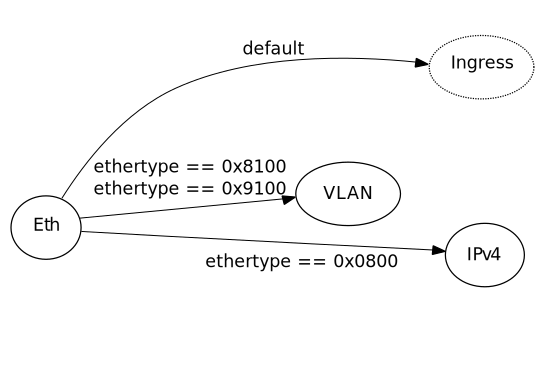
\includegraphics[scale=0.52]{chapters/pic/EthernetParseGraph.eps}
    \caption{Graphical representation of \textit{parse\_ethernet}.}
    \label{fig:parseEthernetRepresentation}
\end{figure}

The second block, \emph{metadata generator}, is used for generation of metadata field values for each processed packet. 
As we proposed before, metadata structure is inferred from Protocol Header declaration because metadata are syntactically defined in the same form. 
Initial values of metadata fields are inferred from Packet Parsed definition using the \textit{set\_metadata} statement. 
Therefore, the \emph{metadata generator} generates the initial values of all required metadata structures as described in P4 program.

Mapping to \emph{check} module is also quite straightforward and intuitive. 
The P4 program allows to define the \textit{field\_list\_calculation} statement which simply binds checksum algorithm to the list of input fields. 
This list is provided in \textit{field\_list} statement. The following example was taken from \cite{p4languagespec}:

\begin{Verbatim}[fontsize=\small]
field_list l3_hash_fields {
    ipv4.srcAddr;
    ipv4.dstAddr;
    ipv4.protocol;
    ipv4.protocol;
    tcp.sport;
    tcp.dport;
}

field_list_calculation ecmp_hash {
    input {
        l3_hash_fields;
    }
    algorithm    : crc16;
    output_width : 16;
}
\end{Verbatim}

The proposed example introduces declaration of L3 hashing, including \textit{ipv4} and \textit{tcp} protocol fields. 
The \emph{check} module setups initial values of control path signals based on result from this stage.
In the case of any error, the processed packet is marked as invalid and the next processing depends on implemented behavior of
Match+Action pipeline elements. 
The general implementation of the \emph{check} module is part of our ongoing research.
%We limit the functionality of the \emph{check} module to setting of initial control path signal values  without any checking of hash fields. 

\subsection{Mapping to Match+Action Group}
\label{sec:mappingControlToMaGroup}
This section introduces the idea for mapping of P4 program to Match+Action processing pipeline. 
The fundamental processing unit of our pipeline is \emph{Match+Action group} which logically unifies complex operations 
like ACL, packet filtering, and so on. 
Some complex programs are divided into more steps because the next step of implemented algorithm depends on the result of previous. 
The P4 language allows to define complex processing program in \textit{control program} statement. 
Each program contains one or more conditional statements (\emph{Match+Action routers}) or table calls (\emph{Match+Action tables}) 
which are connected into deep pipeline. Each \emph{Match+Action table} has three functionalities: (1)~mapping of headers and 
metadata fields to most suitable action, (2)~modification of protocol headers and metadata fields based on selected action and 
(3)~selection of next Match+Action element in processing pipeline. 
The P4 language allows to define the structure of \emph{Match+Action table} using the \textit{table} statement. 
Each P4's table statement contains two declarations: (1)~\textit{reads} statement which defines the structure of search key 
(i.e., it defines a list of used protocols/metadata fields together with matching algorithms) and 
(2)~\textit{actions} statement which defines a list of allowed actions. The simple filtering in P4 language looks like this:
\begin{Verbatim}[fontsize=\small]
// Filter table.
table filter {
    reads {
        ipv4.srcAddr : lpm;
    }
    actions {
        _permit;
    }
}

//Drop table (no read block => just run the action)
table drop {
     actions{
        _drop;
    }
}

// Filtering program
control ingress {
    // Drop all non-IPv4 traffic
    if(valid(ipv4)) {
        // Try to find the rule 
        apply(filter) {
           //Table miss  = drop packet
            miss {apply(drop);}
        }
      } else {
          // non-IPv4 traffic has been detected
          apply(drop);
      }
}
\end{Verbatim}

The proposed example introduces two tables --- \textit{filter} and \textit{drop}. The first table, \textit{filter}, defines the used protocol field 
and possible action (\textit{\_permit} in our case). The second table, \textit{drop}, defines one possible action 
(\textit{\_drop)} and no matching field. In such case, the P4 defines to use the default action. 
The \textit{control program} defines the order of Match+Action elements in the processing pipeline. 
In our case, we start with evaluation of \textit{if-else} statement which drops all non-IPv4 traffic by execution of drop table. 
The conditional statement is mapped to \emph{Match+Action router}. Each IPv4 packet is passed to the
\textit{filter} table which is followed by the \textit{drop} table in the case of table miss (in \textit{filter}).
The text provides two graphs. The Fig.~\ref{fig:grapIpv4Program} represents the graph of control program and 
Fig.~\ref{fig:matchActionIpv4Program} shows the structure of Match+Action pipeline.

\begin{figure}[h]
    \centering
    \includegraphics[scale=0.45]{chapters/pic/filter-control-program-graph}
    \caption{Graph of \textit{ingress} control program.}
    \label{fig:grapIpv4Program}
\end{figure}

The proposed example demonstrates the main idea for mapping from P4 language to pipeline of Match+Action elements. 
That is, \textit{control program} defines the \emph{Match+Action group}, all tables in a group are mapped to \emph{Match+Action tables} and all 
conditional statements are mapped to \emph{Match+Action router}.
We provide more details about the transformation of P4 program to Match+Action element pipeline in Chapter~\ref{chap:matchActionProcessing}.

\begin{figure}[h]
    \centering
    \includegraphics[scale=0.45]{chapters/pic/filter-control-program-pipeline}
    \caption{Match+Action pipeline structure of \textit{ingress} control program.}
    \label{fig:matchActionIpv4Program}
\end{figure}

\subsection{Mapping to Checksum Update and Deparser}
This section demonstrates the idea for mapping from P4 program to \emph{checksum update} and \emph{deparser} module. 
Firstly, we start with  introduction of \emph{checksum update}. The idea for mapping is similar to mapping of P4 program to \emph{check} module
(see Sec.~\ref{sec:mappingToParserMetadataCheck} for more details). 
This module also uses P4's \textit{field\_list\_calculation} statement for update of hash fields because some data may have changed 
in Match+Action processing pipeline. The general structure of this module is part of our ongoing research. 

The last module, \emph{deparser}, is the output module in proposed pipeline architecture. 
The main function of this module is to construct the output packet from incoming header fields.
\textit{Deparser}'s behavior is inferred from P4's Header Format and Packet Parser definition because deparser performs inverse operation to parsing.  
We don't discard any metadata from the processing pipeline and we transfer all fields to the output together with constructed packet. 
These metadata fields are used by other blocks after the deparser. 
We provide more details about the transformation of P4 program to \emph{deparser} in Sec.~\ref{sec:deparserArch}.

\section{Summary}
% Popsali jsme zakladni strukturu a v dalsi casti textu se budeme venovat zakladnim blokum (parser, deparser, match+action tabulky)
The chapter introduces target architectures for mapping of P4 program. 
Firstly, the text introduces not only state-of-the-art software based targets, but also more powerful hardware targets including NPUs and FPGAs.
We selected the FPGA as our target architecture because it connects the flexibility of software with parallel nature of hardware into one
compact package (i.e., the functionality of the hardware can be reprogrammed). 

Secondly, we introduced the architecture of our high-speed processing pipeline (published in \cite{2016h2rc-p4}).
The main idea of the architecture is based on the Parser-Deparser model (published in \cite{2016MicproP4}) which is flexible and suitable 
for implementation of general packet processing engine in hardware.
We demonstrate the flexibility of this approach on two common use cases --- VLAN tagging and network traffic analysis.
Finally, the last section introduces ideas for mapping of P4 language constructs
to our high-speed pipeline architecture. %, including references to following text of this thesis.
